
%
% Chapter 2
%

\chapter{Theoretical bases}
\label{chap:theory}
In this chapter we describe the theoretical motivations that drive the searches described in this thesis. We start with a description  the standard model (SM), its particle content and interactions and the Higgs mechanism. We then talk about the inadequacies of the SM, and the existence of physics beyond the standard model (BSM). We then outline a few BSM models and how they point towards the possibility of the decays that we search for in this thesis.  

\section{The Standard Model }
\label{sec:SM}
The SM is the result of human endeavors over centuries to understand what we and the world around us are made of, and capture those ideas in beautiful mathematical form. Our understanding of the world around us has refined progressively from the ancient times, when best tools of observation we had were nothing but our own eyes to the current day when we are able we collide particles that make up matter at unprecedented speeds, and have sophisticated tools like the CMS detector to aid us. From the ancient greeks who pondered over philosophical questions about what the basic elements of nature were, to the discovery of electron in 1898 by J.J.Thompson, to Rutherford's famous gold foil experiment, to the discovery of the neutron by James Chadwick in 1932 have been stepping stones towards our understanding of nature and the formulation of SM. During the course of its formulation and after, the SM has accurately explained phenomena alreafy known and  predicted the existence of particles that were discovered later. The last of these particles is the Higgs Boson, discovered in 2012 at CERN by the CMS and the ATLAS experiments~\cite{Aad:2012tfa, Chatrchyan:2012ufa, Chatrchyan:2013lba}. The SM is a gauge theory, in which three of the four known natural forces (strong, electromagnetic, weak and not gravity~\ref{tab:forces}) are represented by the SU(3)xSU(2)xU(1) symmetry group. This symmetry group describes under which transformations the SM is invariant. By Noether's theorem each of the above symmetries associated with the SM Lagrangian is associated with a conserved quantity: color charge, weak isospin and electric charge. The following describes the elementary particles of the SM, the interactions among these and finally, the spontaneous symmetry breaking mechanism.

\subsection{Elementary particles}
There are two kinds of elementary particles in the SM. They are characterized by the intrinsic angular momentum that they carry, i.e. by their spin. Fermions, which has half-integer spins, form the building blocks of matter. Bosons, which have integer spins, are the force-carriers or mediators of interactions.
\subsubsection{Fermions of SM}
Fermions are fundamental particles, i.e. they cannot be broken down into further consituents. The space-time evolution of the fermions is described by the Dirac equation and their behavior follows Fermi-Dirac statistics. All fermions are subject to the Pauli exclusion principle. The fermions can be further categorized into two classes depending on their interaction with the strong force. Fermions wich do not interact with the strong force are called leptons, and do not carry any color charge. Quarks carry color charge and interact via the strong force. Both leptons and quarks are further classified into three generations. Each lepton generation consists of a lepton and a neutrino while each quark generation consists of a up type and a down type quark. These are outlined in detail below.

Leptons comprise of the familiar electron (e), its heavier cousins muon ($\Pgm$) and tau lepton ($\Pgt$) which carry the same negative electric charge as the electron ($1.6\times10^{-19} C$).  The heavier leptons $\Pgt$ ($\sim 1.8\,\mathrm{GeV}/c^2$ ) and $\Pgm$ ($\sim 105.7\,\mathrm{MeV}/c^2$) have short lifetimes of $\sim 2.9\times 10^{-13}\,$s and $\sim 2.2\times 10^{-6}\,$s respectively. The eventually decay into an electron which is the lightest lepton ($\sim 0.5\,\mathrm{MeV}/c^2$ ) and has infinite lifetime, or lighter hadrons. In the CMS detector, the $\mu$ survives long enough to reach the muon systems is thus detected as its own distinct signature. The $\Pgt$ on the other hand, owing to its extremely short lifetime, can travel only a very short distance ($\sim <10\,mm$) before decaying. Thus, only decay products of tau leptons are able to be directly detected by CMS. Each charged lepton is associated with an electrically neutral neutrino. They are called electron neutrino ($\nu_e$), muon neutrino ($\nu_{\mu}$) and tau neutrino ($\nu_{\mu}$). Because neutrinos carry no electric charge, they do not interact via electromagnetic interaction. This means the only way they interact is via the weak interaction. This makes neutrinos are very difficult to detect. In particular, they pass through the CMS detector effectively without interacting at all, and their presence and the energy they carry can only be estimated using imbalance in transverse momentum of observed particles (see section~\ref{mt_met_recon}). The three generations of leptons are pictorially shown below. 

\begin{equation*}                                                                                                                           \binom{e^{-}}{\nu_{e}} \;\;\; \binom{\mu^{-}}{\nu_{\mu}} \;\;\; \binom{\tau^{-}}{\nu_{\tau}}                                             \end{equation*}

Quarks come in two generations: up-type and down-type. The up-type quarks are the up quark (u), charm quark (c) and top quark (t). Their down-type counterparts are down quark (d), strange quark (s) and bottom quark (b). Each up-type quark carries a negative electric charge of 2/3 times the charge of the electron. Each down-type quark carries a negative charge of 1/3 times the charge od the electron. Just like the leptons, each progressive generation is heavier with the third generation consisting of the top and bottom quarks being the heaviest. In fact, the top quark was the last of the SM fermions to be discovered in 1995, and is the heaviest particle in the SM ($\sim 173\,\mathrm{GeV}/c^2$). As mentioned above, all quarks carry color charge. Color charge is to strong force as electric charge is to electromagnetic force. This allows quarks to interact via the strong force. Due to a phenomenon called color confinement, quarks aggregate together into colorless (having zero color charge) particles called hadrons. Hadrons are either formed of 3 (anti-)\,quarks (baryons) or 2 (anti-)\,quarks (mesons). The proton and neutron are baryons. It is made of two up quarks, and one down quark. It has a mass of $\sim 938.3\,\mathrm{MeV}/c^2$ and is stable (infinite lifetime). The neutron is made of one up quar and two down quarks. It has a mass of $\sim 939.5\,\mathrm{MeV}/c^2$ and has a lifetime of $\sim880\,$s. The three generations of quarks are pictorially shown below.

\begin{equation*}                                                                                                                          \binom{u}{d} \;\;\; \binom{c}{s} \;\;\; \binom{t}{b}                                                                                      \end{equation*}

Each particle described above has an anti-particle associated with it. Particles (matter) and their anti-paritcles (anti-matter) are almost identical except they have opposite physical charges (electric charge, color charge). For example, The anti-particle of an electron is the positron which is nearly identical to the electron except for the fact that it has positive electric charge.

\subsubsection{Bosons of SM}
The bosons in SM are carriers or mediators of force. Their behavior follow bose-einstein statistics and they are not constrained by the Pauli exclusion principle. The strong interaction, as its name suggests, is the strongest of the fundamental forces\,(~\ref{tab:forces}). The eight gluons mediate the strong interactions between particles with color charge. Photons are the mediators of the next strongest fundamental forece, the electromagnetic force. Gluons and photons are massless, electrically neutral and have spin 1. Additionally, gluons carry color charge. This is in contrast to photons which are electrically neutral. The $\mathrm{W}^+$,$\mathrm{W}^-$ and Z gauge bosons mediate the weak interactions between particles of different flavors. Both bosons have spin 1. However, unlike the photons and the gluons, they are heavy. The W boson has a mass of $\sim 80.4\,\mathrm{GeV}/c^2$ and the Z boson has a mass of $\sim 91.2\,\mathrm{GeV}/c^2$. Finally, the Higgs boson which is a massive, scalar (spin 0) and electrically neutral boson is responsible for giving masses to W, Z bosons and fermions.         

\begin{table}[hbtp]
\begin{center}
\caption{Relative strengths and ranges of all four fundamental forces, with the strong force as the baseline.}
\begin{tabular}{|cccc|}
\hline
Interaction & Relative Strength & Range \\
\hline
Strong & $10^{39}$ & $10^{-15}\,m$\\
Electromagnetic & $10^{36}$& $\infty$\\
Weak &  $10^{25}$ &$10^{-18}\,m$\\
Gravity & $1$ &$\infty$\\
\hline
\end{tabular}
\label{tab:forces}
\end{center}
\end{table}

A pictorial summary of all particles in the SM, divided into different classes is shown in Figure~\ref{fig:sm_zoo}.

\begin{figure}[hbtp]
 \begin{center}
   \includegraphics[width=0.8\textwidth]{plots_and_figures/chapter2/SM_particles.pdf}
   \caption{A pictorial summary of particles in the SM. The Higgs boson is shown in yellow. Gauge bosons are shown in red. Leptons and quarks are shown in green and violet respectively~\cite{sm_zoo}.\
.}
   \label{fig:sm_zoo}
 \end{center}
\end{figure}


\subsection{Theory of interactions}
The SM follows the Lagrangian formalism to describe interaction between the particles. Given the SM is a gauge theory, symmetries of the Lagrangian are central to its understanding. In a gauge theory, the Lagrangian is invariant under certain (groups of) transformations and each such symmetry is associated with a conservartion law (Noether's theorem). The underlying symmetry group that the SM Lagrangian is invariant under is SU(3)xSU(2)xU(1), where the group SU(3) corresponds to the strong interaction while the group SU(2)xU(1) corresponds to theelectromagnetic and weak (electroweak) interaction. Each of the group generator is associated with an underlying vector field, the quanta of which are the gauge bosons (gluons, photons, W and Z) described above. We describe the SM interactions briefly below in order of strength.

\subsubsection{Strong and Electroweak interactions}
The theory that describes the strong interaction is called Quantum Chromodynamics (QCD). It is a non-abelian gauge field theory based on  SU(3) symmetry. Color charge is the quantity conserved under this symmetry. There are three colors: green (g), red (r) and blue (b). Each color has a corresponding anticolor (negative color). As noted earlier, all quarks and gluons have non-zero color charge. Quarks carry a single color, while each of the eight gluons have a color and anticolor charge. The theory being non-abelian, the generator matrices (Gell-Mann matrices) do not commute. The consequence of this is that gluons (unlike photons) can interact with each other.

The theory that was originally formulated to describe the electromagnetic interaction is called Quantum Electrodynamics (QED). It is a gauge field theory based on U(1) symmetry. Electric charge is qunatity conserved under this symmetry and all particles that interact via electromagnetic interaction need to carry electric charge. Unlike the gluons, the photon (because it is electrically neutral) cannot interact with itself. The weak interaction was initially formulated based on the SU(2) symmetry group, with conserved quantity being the weak isospin. The associated gauge bosons are massive and can be electrically neutral (Z) or charged (W). Quarks of (same) different generations can interact with each other via (Z) W bosons. In the 1960s Glashow, Salam and Weinberg combined the theories describing electromagnetic and weak interactions, after realising that they were different aspects of the same overarching interaction. This is regarded as electroweak unification, and the electroweak interaction is described by a guage field theory based on combined SU(2)xU(1) symmetry group. The conserved quantitites, weak isospin (T) and electric charge (Q) are related via:

\begin{equation*}
  Q = T_{3} + \frac{Y_{W}}{2}
\end{equation*}
, where $\mathrm{T}_{3}$ is the third component of T and $\mathrm{Y}_{W}$ is a quantum number called the weak hypercharge.

The gauge bosons, in this theory, are divided into a triplet with two electrically charged and one neutral component (corresponding to Ws and Z), and a singlet with no electric charge (corresponding to the photon). However, in order to maintain gauge invariance of the theory, no mass terms are allowed in the Lagrangian. This would require ALL the gauge bosons (and fermions) to be massless. This is known not to be the case. This broken symmetry (photons being massless and W/Z bosons being massive) is explained by the Higgs mechanism, described in the next section.

\subsubsection{The Higgs mechanism}
In order to explain how massive gauge bosons come about, the idea of electroweak spontaneous symmetry breaking (EWSB) is introduced. The phenomenon by which EWSB is utilized to give mass to particles is called the Higgs mechanism. Under this mechanism, a new scalar field ($\phi$) called the Higgs field and an associated potential V$(\phi))$ is introduced. This is represented as doublet and has four degrees of freedom. Three of these four degrees of freedom correspond to the polarizations of the massive W and Z bosons. In order for the Higgs field to interact with W and Z but the not the photon, symmetry has to be broken. The minimum of the potential, i.e. the vacuum state or ground state must be non-zero for this to happen. The parameters of V$(\phi))$ is so chosen that it has a Mexican-hat (sombrero) shape, which has infinite degenerate non-zero minima. This non-zero minimum is called the vacuum expactation value (vev), which is measured to be 246\,GeV. The direction of symmetry breaking is such that it gives mass to the Z boson but leaves the photon massless. This breaking of symmetry is called spontaneous because there is no particular reason for this direction have been picked. Nature just happened to spontaneously pick this direction. The Higgs field gives rise to a new massive scalar particle. This particle is the Higgs boson, and corresponds to the fourth remaining degree of freedom of the scalar doublet mentioned above. The fermions acquire mass via Yukawa interaction of the Higgs boson. The strength of the Yukawa coupling of the Higgs boson with fermions is proportional to the fermion masses. To summarize, the Higgs mechanism allows the introduction of a mass term for the gauge bosons without breaking the underlying gauge symmetry of the SM Lagrangian. Addition of this field, gives rise to another massive particle, the interactions with which give masses to gauge bosons and fermions. This massive particle is a scalar boson called the Higgs boson, which was discovered in 2012 at CERN by CMS and ATLAS, 50 years after it was first predicted to exist. Before the LHC, experiments at LEP and Tevatron looked for existence of the Higgs boson. It was the last missing piece of the SM, and its discovery can be thought to conclude an era in particle physics and lead us into a newer equally exciting era.


\subsection{Higgs Boson production and decays at the LHC}
There are several different ways the Higgs boson can be produced at the LHC. The LHC collides protons at high energy, and the production modes of the Higgs boson, in order of cross-section, at the LHC are :

\begin{itemize}%[itemsep=5pt]
\item \textbf{Gluon-Gluon Fusion (ggH)}: Since gluons are massless, they do not directly couple to the h. This production mode proceeds via quark loop. The ggH production cross-section at 13 TeV is $\sim48.37\,pb$ at N3LO~\cite{YR4}. 
\item \textbf {Vector Boson Fusion (VBF)}: This production mode has the second largest cross section at the LHC. This mode is characterized by two high-momentum quarks in the final state which hadronize to form jets. The VBF production cross-section at 13 TeV center-of-mass energy is $\sim3.77\,pb$ at NNLO.
\item \textbf {Associated Production}: The third largest h production mode at the LHC involves the production of a virtual $W^*/Z^*$ boson that splits into a real boson W/Z boson and a h. The WH production cross-section is  $\sim1.36\,pb$ and the ZH production production cross-section is $\sim0.87\,pb$, at NNLO level for a center-of-mass energy of 13 TeV at the LHC.
\item \textbf {ttH Production}:   In this production mode, the h is produced in along with a pair of top quarks. The production cross-section at 13 TeV center-of-mass energy is $\sim0.50\,pb$ at NLO.
\end{itemize}
  
The Feynman diagrams for h production modes described above are shown in Figure~\ref{fig:higs_feyn}. The cross-section of each process as a fuction of center-of-mass energy is shown in Figure~\ref{fig:higs_xs_som}.


\begin{figure}[hbtp]
 \begin{center}
   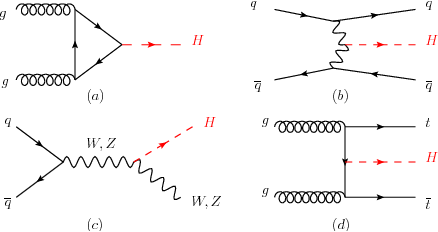
\includegraphics[width=0.95\textwidth]{plots_and_figures/chapter2/higgs_prod.png}
   \caption{ Feynman diagrams for Higgs production modes at LHC: (a) gluon-gluon fusion, (b) vector boson fusion,(c) associated production and (d) ttH~\cite{higg_prod}.}
   \label{fig:higs_feyn}
 \end{center}
\end{figure}


\begin{figure}[hbtp]
 \begin{center}
   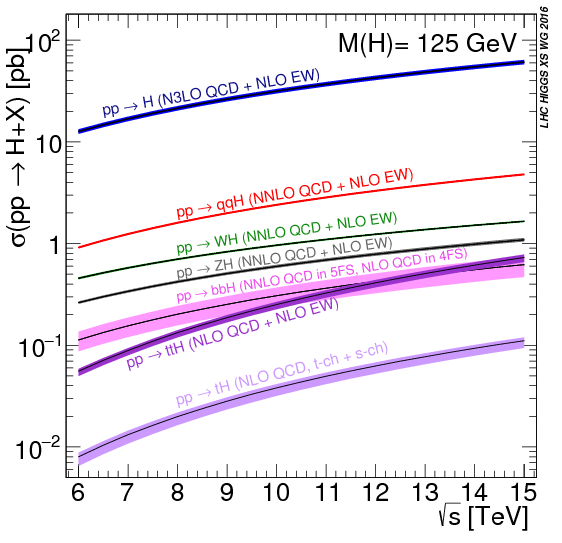
\includegraphics[width=0.8\textwidth]{plots_and_figures/chapter2/higgs_xs.png}
   \caption{The SM Higgs boson production cross-section as a function of the center-of-mass energy in proton-proton collisions at the LHC~\cite{higg_prod}.}
   \label{fig:higs_xs_som}
 \end{center}
\end{figure}
    







\section{Physics beyond the standard model}
\label{sec:BSM}

